% Informe de la Tarea 2 (Hidrología, 202602), grupo G01.
% Compilar desde esta carpeta:  latexmk -pdf informe.tex   (o pdflatex + bibtex + pdflatex x2)
% y copiar informe.pdf a la raíz de la entrega como T2_202602_G01_informe.pdf.
% Las figuras se leen de productos/ (rutas relativas). Los recuadros \pendiente{...} marcan lo que falta escribir:
% el informe no se entrega con ninguno.
\documentclass[11pt,letterpaper]{article}
\usepackage[utf8]{inputenc}
\usepackage[T1]{fontenc}
\usepackage[spanish,es-noshorthands,es-nodecimaldot,es-tabla]{babel}
\usepackage{lmodern}
\usepackage[margin=2.5cm]{geometry}
\usepackage{graphicx}
\usepackage{booktabs}
\usepackage{amsmath}
\usepackage{siunitx}
\sisetup{output-decimal-marker={.}, group-separator={\,}, group-minimum-digits=4}
\usepackage{xcolor}
\usepackage[most]{tcolorbox}
\usepackage[round,authoryear]{natbib}
\usepackage{url}
\usepackage[hidelinks]{hyperref}
\usepackage{caption}
\captionsetup{font=small,labelfont=bf}

\graphicspath{{../../productos/punto1/}{../../anexos/punto1/}{../../productos/punto2/}}

% Recuadro para lo que falta: no debe quedar ninguno en la versión entregada.
\newtcolorbox{pendientebox}{colback=orange!8,colframe=orange!70!black,boxrule=0.6pt,arc=2pt,
  left=4pt,right=4pt,top=2pt,bottom=2pt,fontupper=\small}
\newcommand{\pendiente}[1]{\begin{pendientebox}\textbf{Pendiente:} #1\end{pendientebox}}

\newcommand{\ETo}{ET$_\mathrm{o}$}
\newcommand{\PM}{Penman--Monteith (FAO-56)}

\title{Evapotranspiración en la cuenca del río Fonce y diseño hidrológico\\[4pt]
  \large Hidrología · Tarea 2 · Semestre 202602 · Grupo G01}
\author{\pendiente{Nombres completos de los tres integrantes (Gómez, Gómez, Na).}}
\date{24 de noviembre de 2026}

\begin{document}
\maketitle

% =====================================================================================================
\section{Introducción}

\pendiente{Punto 1: la cuenca del río Fonce hasta San Gil (IDEAM 24027010, \SI{2098.85}{km^2}, de 1\,118 a
4\,284~m), su contexto hidroclimático (de la ficha de la Tarea 1), la motivación, los objetivos y las preguntas o
hipótesis, con bibliografía. Las cinco preguntas de la síntesis pueden servir de preguntas iniciales: cuál es la
demanda y qué la controla; cuánta agua devuelve la cuenca y con qué incertidumbre; en qué meses manda la energía y en
cuáles el agua; qué ha cambiado y por qué; qué proceso distingue a la cuenca.}

\pendiente{Punto 2: el sitio, su contexto y las preguntas (lo escribe la compañera).}

% =====================================================================================================
\section{Metodología}

\subsection{Punto 1: evapotranspiración en la cuenca del Fonce}

\paragraph{Datos y periodo.} Se trabajó en 1998--2022 (25 años), el periodo de IMERG en la Tarea 1; las tendencias
de la Tarea 1 empiezan en 1981 y las de este trabajo no. La cuenca es el polígono de CAMELS-COL hasta San Gil
\citep{camelscol}. Los forzantes de la \ETo{} son series horarias de ERA5-Land \citep{munoz2021}, del producto de
series de tiempo, en 6 centros de celda de 0.1° con al menos el 90~\% de su área dentro de la cuenca, uno por
franja de altura de igual área (1\,580 a 3\,259~m). El valor de cuenca es el promedio ponderado por Voronoi. Los días
se arman en hora local (UTC$-5$). La lluvia y el caudal vienen de la Tarea 1: PI (IMERG ponderado por área de celda;
\citealp{huffman_imerg}), PL (7 pluviómetros del IDEAM dentro de la divisoria, depurados) y Q observado en San Gil, en
lámina. La lluvia principal es $\bar{P} = (\mathrm{PI}+\mathrm{PL})/2$; PI y PL quedan como sensibilidad. De DHIME
(IDEAM) se usaron brillo solar, Tmáx, Tmín y HR de Mogotes, La Sierra y Charalá, y el viento de Mogotes-AUT. Los
productos de ET real son GLEAM v4.3a \citep{miralles2025}, MOD16A2GF v061 \citep{running2021}, SSEBop v6.1 y v5
\citep{senay2013,senay2023}, TerraClimate \citep{abatzoglou2018} y la evaporación de ERA5-Land, promediados en la
cuenca por el área de intersección de cada celda. El ERA5-Land mensual está dañado en sep--dic de 2022
\citep{ecmwf2024}: lo que lo usa se corta en 2022-08; la \ETo{} no está afectada. No hay torre de flujo en la región,
y el tanque evaporímetro de Mogotes-AUT no se usa porque no tiene un factor de unidades coherente.

\paragraph{\ETo{} de referencia.} \PM{}, ec.~6 de \citet{allen1998}, diaria por punto: $T = (T_\mathrm{máx} +
T_\mathrm{mín})/2$; $e_s$ con la media de $e^\circ(T_\mathrm{máx})$ y $e^\circ(T_\mathrm{mín})$; $e_a$ como promedio de
las 24 $e^\circ(T_d)$ horarias; $\gamma$ con la presión de cada punto; $u_2 = 0.748\,u_{10}$ (ec.~47); $G = 0$; $R_n$
del pasto de referencia (albedo 0.23). La \ETo{} mensual es la suma de las diarias. La ec.~47 supone un perfil
logarítmico neutro sobre pasto de 0.12~m: $u_2$ es el viento del pasto de referencia, no el real. Un día a mano
(2010-02-15, punto 6) reproduce el código a 4 decimales.

\paragraph{Pruebas de la referencia.} (1) Rs de estación con Angstrom (FAO-56 ec.~35) frente a la celda de ERA5-Land
de cada estación. (2) \ETo{} \PM{} con datos de estación y viento de Mogotes-AUT medido a 10~m
\citep{ideam_gdim003}, solo en días con todas las entradas. (3) La pet de TerraClimate, ASCE Penman--Monteith con
resistencia corregida por CO$_2$ \citep{yang2019}; sus anomalías vienen de ERA5. La dispersión entre pruebas, por mes,
es $|$sesgo~\% frente a TerraClimate $-$ media del sesgo~\% frente a las 3 estaciones$|$.

\paragraph{Métodos de otras familias.} Thornthwaite \citep{thornthwaite1948}, Hargreaves \citep{hargreaves1985},
Priestley--Taylor \citep[$\alpha = 1.26$;][]{priestley1972}, Makkink \citep{makkink1957}, Cenicafé
\citep{jaramillo2006}, Penman en la forma de FAO-24 con $c = 0.8$ \citep{penman1948,doorenbos1977} y la relación
complementaria de \citet{brutsaert1979}, con las ecuaciones de las notas del curso \citep{hoyos_et}. Mismos forzantes,
periodo y paso diario que la \ETo. Cada método se compara, sin calibrar, con una referencia de su misma superficie:
\PM{} para los de pasto (y Thornthwaite, que no tiene conversión), \PM{} con $r_s = 0$ para Priestley--Taylor.

\paragraph{Explicación de las diferencias.} Términos radiativo y aerodinámico de la ec.~6; $\alpha^* =
\mathrm{ET_o}/E_\mathrm{eq}$; y un experimento de sensibilidad: Tmáx y Tmín $+1$ y $+2$~°C (con $e_a$ constante y con
HR constante), $u_2$ $+10$~\%, Rs $-10$~\% y $e_a$ $+10$~\%.

\paragraph{ET real.} Balance $\mathrm{ET} = \bar{P} - Q$ en años calendario ($\Delta S$ del suelo de ERA5-Land
$\approx 0$ en el largo plazo). Incertidumbre al 95~\%: $\sigma_P = 1.96\,|\mathrm{PL}-\mathrm{PI}|/2$, $\sigma_Q =
25.6$~\% de Q \citep{dibaldassarre2009} y $\sigma_\mathrm{ET} = \sqrt{\sigma_P^2 + \sigma_Q^2}$. Techo de energía
$R_n/\lambda$ con la $R_n$ real de ERA5-Land. Un producto es consistente con el balance si cae dentro de
$\pm\sigma_\mathrm{ET}$.

\paragraph{Régimen.} Espacio de Budyko con $\bar{P}$ ($\varphi = \mathrm{ET_o}/P$, $\varepsilon = \mathrm{ET}/P$),
curva de Fu y elasticidad de Q a P \citep{sankarasubramanian2001}; $\varphi$ mensual; y fracción evaporativa
$\lambda\mathrm{ET}/R_n$ frente a la humedad del suelo de GLEAM \citep{seneviratne2010}.

\paragraph{Cambios en la demanda.} Tendencias 1998--2022 de la \ETo, Thornthwaite, T, $e_a$, $u_2$ y Rs con los
métodos de la Tarea 1: Mann-Kendall estacional con pendiente de Sen (p por permutación de años), OLS con una constante
por mes y error de Newey-West (12 rezagos), Pettitt y control de FDR; $\alpha = 0.05$.

\pendiente{Juan: revisar y pasar a su voz (borrador en \texttt{anexos/borrador\_metodologia.md}). Falta la fase 9
(tema del paisaje).}

\subsection{Punto 2}
\pendiente{Metodología del punto 2 (compañera).}

% =====================================================================================================
\section{Resultados y discusión física}

\subsection{Punto 1}

\subsubsection{La demanda: \ETo{} de referencia}
\begin{figure}[htbp]\centering
  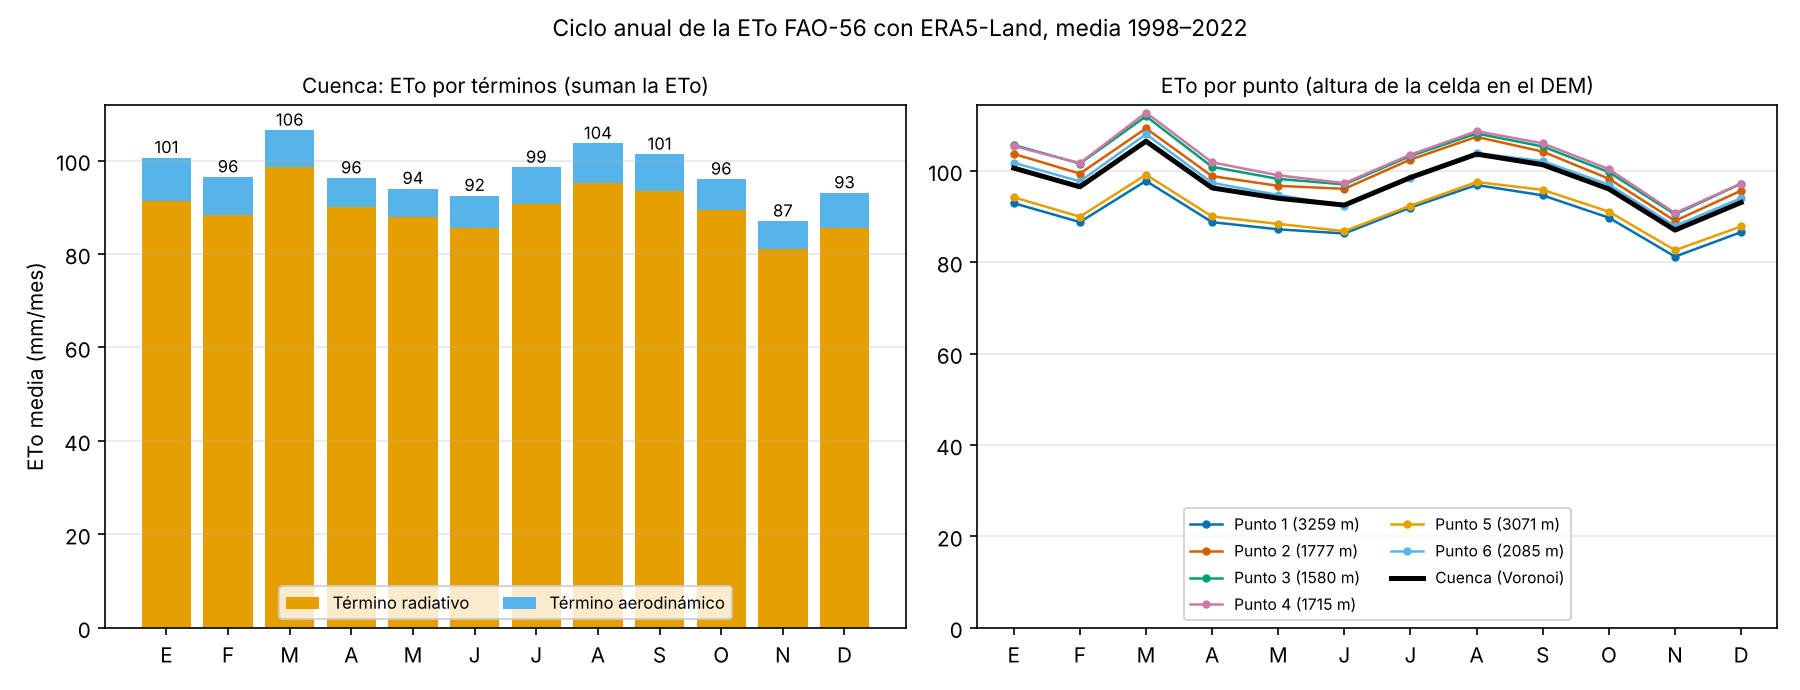
\includegraphics[width=0.9\textwidth]{eto_ciclo_anual.png}
  \caption{Ciclo anual de la \ETo{} \PM{} de la cuenca (media 1998--2022) y sus términos radiativo y aerodinámico.}
  \label{fig:eto_ciclo}
\end{figure}
\pendiente{Juan: valor anual de la \ETo, su ciclo (Fig.~\ref{fig:eto_ciclo}) y qué la controla.}

\subsubsection{¿Qué tan buena es la referencia?}
\begin{figure}[htbp]\centering
  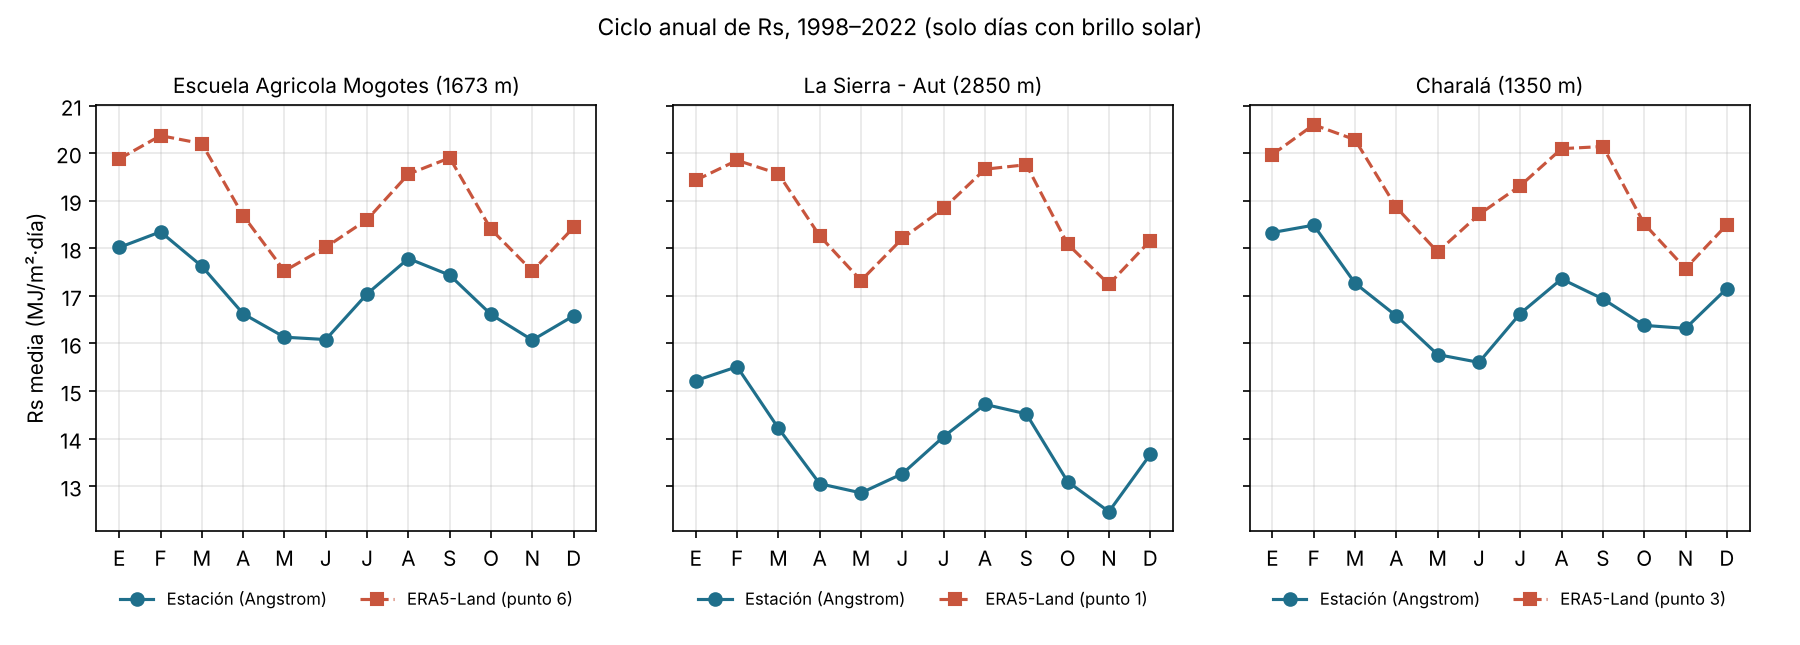
\includegraphics[width=0.48\textwidth]{rs_estaciones_vs_era5land_ciclo_anual.png}\hfill
  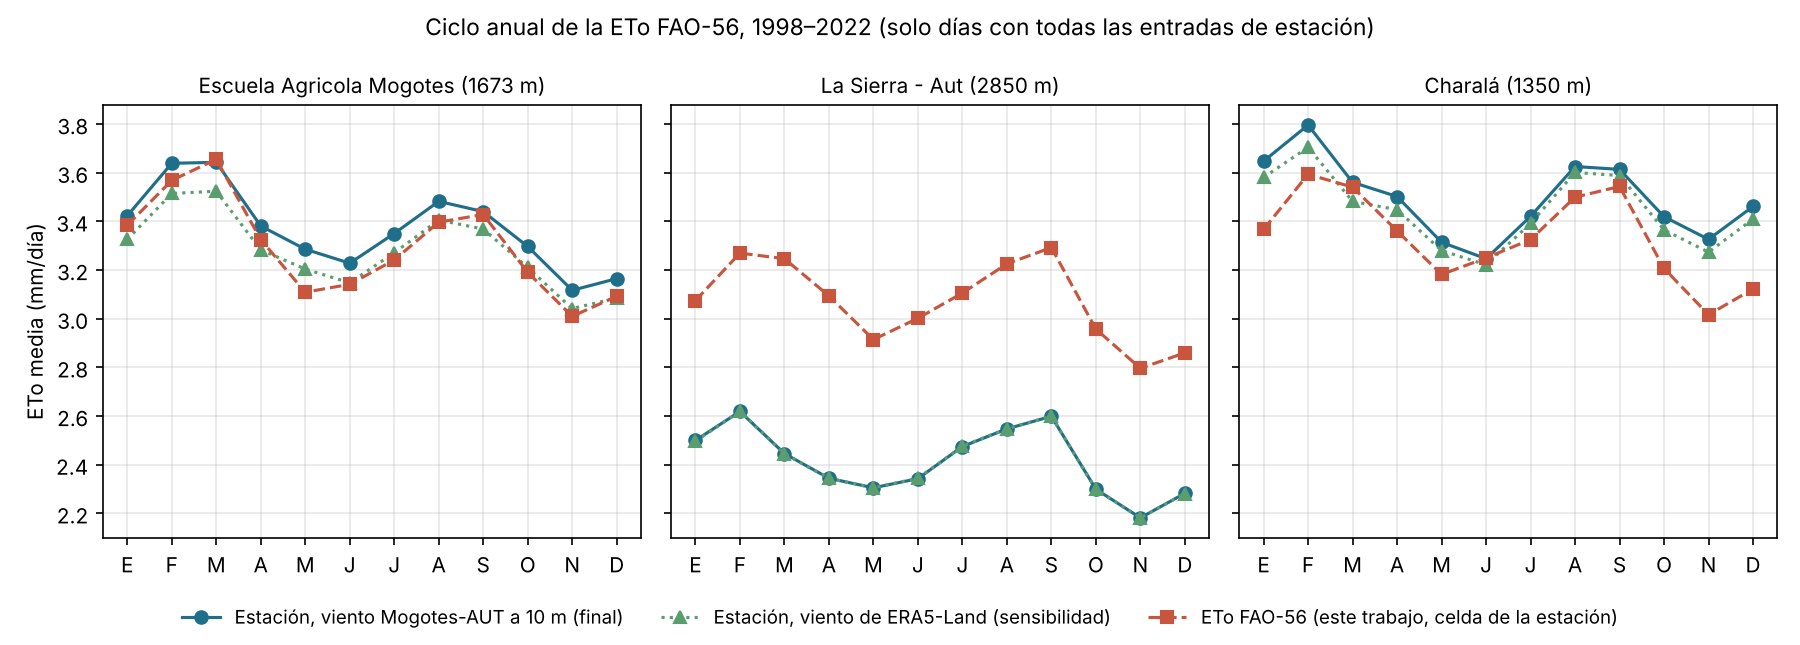
\includegraphics[width=0.48\textwidth]{eto_estaciones_vs_era5land_ciclo_anual.png}
  \caption{Izquierda: Rs de ERA5-Land frente a la de Angstrom en tres estaciones. Derecha: nuestra \ETo{} frente a la
  \ETo{} de estación.}
  \label{fig:pruebas_estaciones}
\end{figure}
\begin{figure}[htbp]\centering
  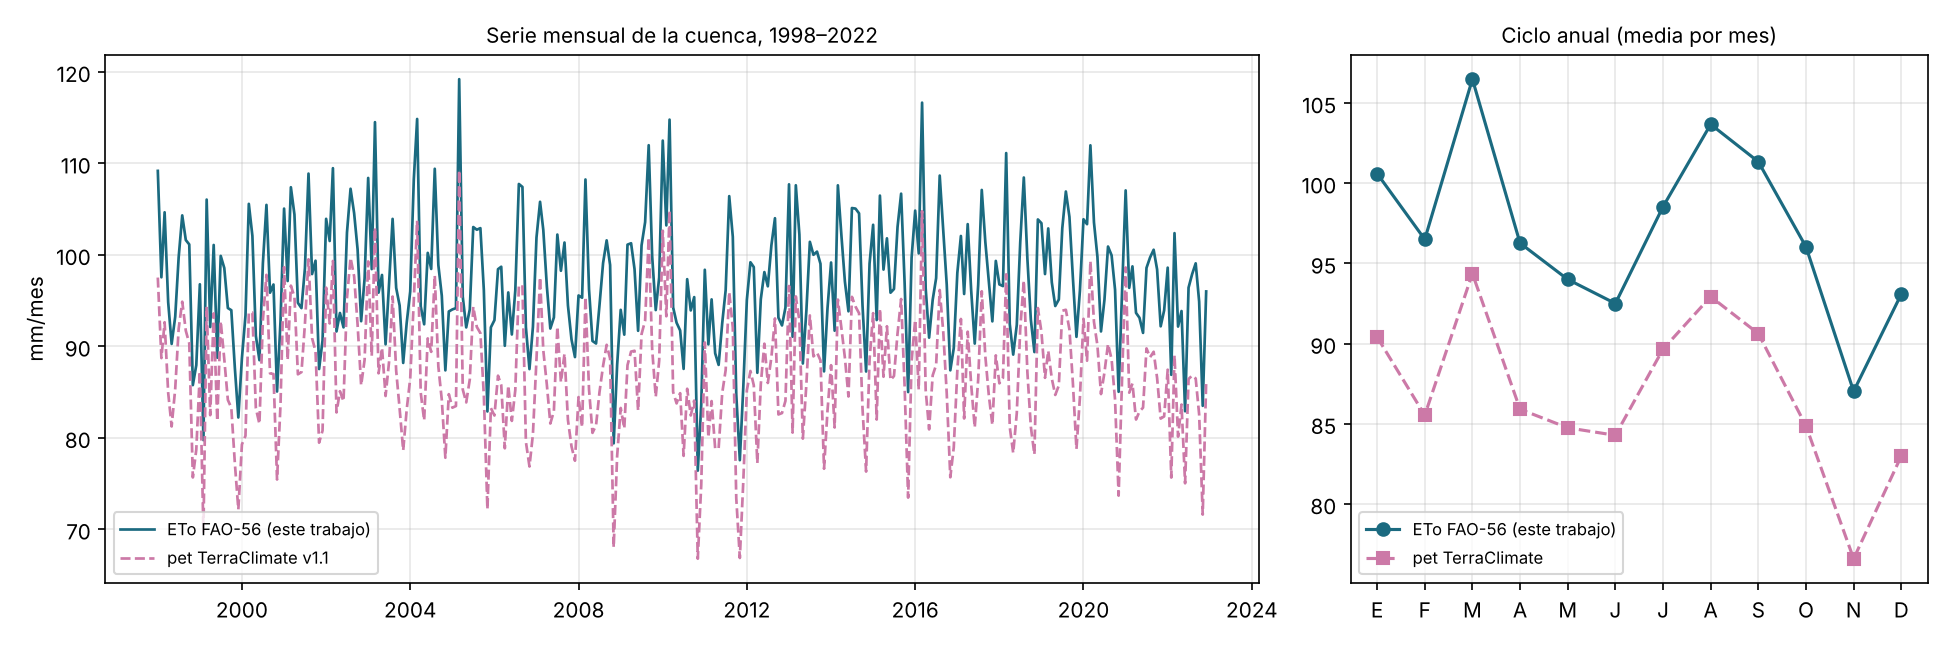
\includegraphics[width=0.8\textwidth]{eto_vs_terraclimate_pet.png}
  \caption{Nuestra \ETo{} frente a la pet de TerraClimate, promedio de la cuenca.}
  \label{fig:terraclimate}
\end{figure}
\pendiente{Juan: resultado de las dos pruebas (Figs.~\ref{fig:pruebas_estaciones} y \ref{fig:terraclimate}), la
dispersión y sus limitaciones.}

\subsubsection{Métodos de otras familias y sus diferencias}
\pendiente{Tabla y figura de los métodos frente a su referencia (hoy solo en el documento de trabajo; falta la
figura fija en \texttt{productos/punto1/}). Punto de control de Juan (fase 4): Makkink es el que mejor se ajusta.}

% Texto de Juan (temp/textos_informe/fase5_diferencias_eto.md), con sus cifras.
\textbf{Penman.} Se calculó con $c = 0.8$, como sugiere FAO-24 (p.~15). Es muy similar al \PM{} con el que se compara
(R$^2$ anual de 0.991), con Penman sistemáticamente por debajo, posiblemente porque el $c$ de FAO-24 puede ser bajo
para esta cuenca. Ambos son adaptaciones del método original de Penman; la diferencia se debe sobre todo al viento y
a la elección de $c$.

\textbf{Makkink.} Usa solo T y Rs: no tiene en cuenta el viento ni la humedad. Funciona bien cuando la humedad no
limita, el viento es bajo y el limitante es la radiación. En la cuenca el término aerodinámico de \PM{} es pequeño y
explica la pequeña diferencia; los coeficientes de Makkink compensan en parte ese término para la zona donde se
calibró.

\textbf{Hargreaves.} Usa Tmáx, Tmín y Ra; sirve cuando hay poca información, como en la Tarea 1. Queda por encima de
\PM{} (+10~\%), posiblemente porque tiende a sobrestimar con HR alta \citep[p.~64]{allen1998}, y la HR media de la
cuenca es 79.3~\%.

\textbf{Cenicafé.} Usa solo la altitud: da una \ETo{} diaria fija. Fue calibrado en los Andes colombianos, incluidas
dos estaciones en Santander, y da una aproximación decente con muy pocos datos ($-12$~\%), pero no sigue las
fluctuaciones.

\textbf{Priestley--Taylor.} No es la ET del pasto de referencia sino la de una superficie húmeda sin $r_s$; por eso se
compara con \PM{} con $r_s = 0$. Las formas son muy similares, con una diferencia estable.

\textbf{Thornthwaite.} Estima la ETP de una superficie con vegetación y sin falta de agua, distinta de la de la \ETo:
la comparación es aproximada. Queda muy por debajo ($-38$~\% en el año). Usa la temperatura como indicador de la
energía; en la cuenca la temperatura es baja por la altitud, no por falta de radiación, así que el método supone poca
energía.

\textbf{$\alpha^*$.} Va de 1.004 (mayo) a 1.028 (enero): casi toda la \ETo{} depende de la energía. El déficit de
vapor y el viento suman entre 7 y 10~\%, y la resistencia del pasto le quita casi todo eso.

\begin{figure}[htbp]\centering
  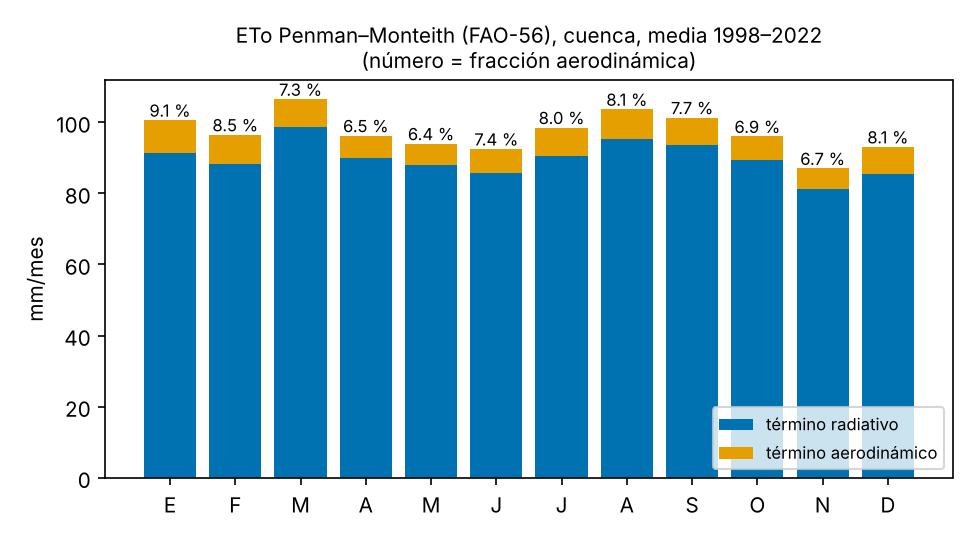
\includegraphics[width=0.48\textwidth]{terminos_fao56.png}\hfill
  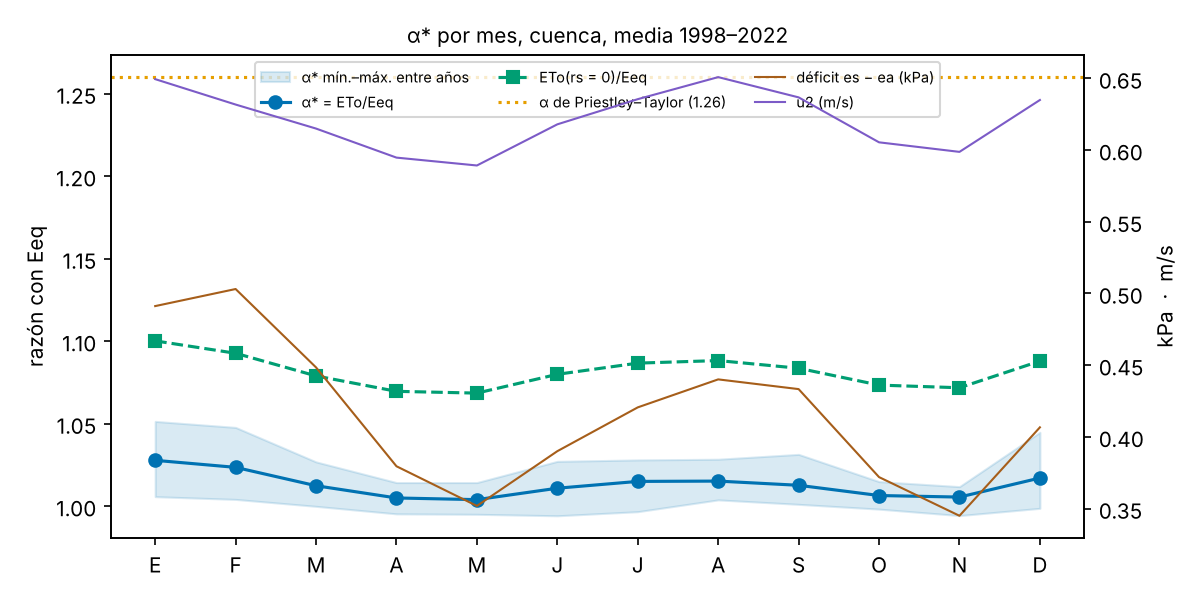
\includegraphics[width=0.48\textwidth]{alfa_implicito.png}
  \caption{Izquierda: términos de la \ETo{} \PM{} por mes. Derecha: $\alpha^* = \mathrm{ET_o}/E_\mathrm{eq}$.}
  \label{fig:terminos_alfa}
\end{figure}
\pendiente{Citar Fig.~\ref{fig:terminos_alfa} en el texto; figura del experimento de sensibilidad (solo está en el
documento de trabajo). Los valores de R$^2$ 0.991 y de las correlaciones de $\alpha^*$ deben salir de un script
(auditoría de las fases 0--5).}

\subsubsection{ET real y su incertidumbre}
\pendiente{Juan: ET = $\bar{P} - Q$ con su $\sigma_\mathrm{ET}$, el techo de energía y los productos (falta la figura
fija de la fase 6 en \texttt{productos/punto1/}).}

\subsubsection{¿Manda la energía o el agua?}
\begin{figure}[htbp]\centering
  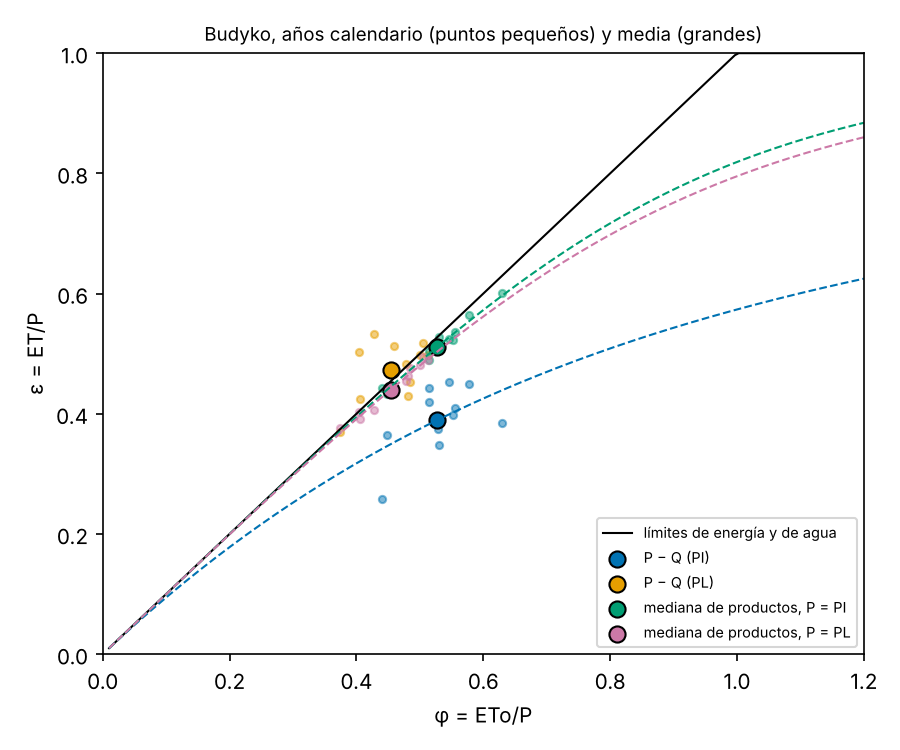
\includegraphics[width=0.7\textwidth]{budyko.png}
  \caption{Espacio de Budyko con $\bar{P}$: años y media, con la curva de Fu ajustada.}
  \label{fig:budyko}
\end{figure}
\begin{figure}[htbp]\centering
  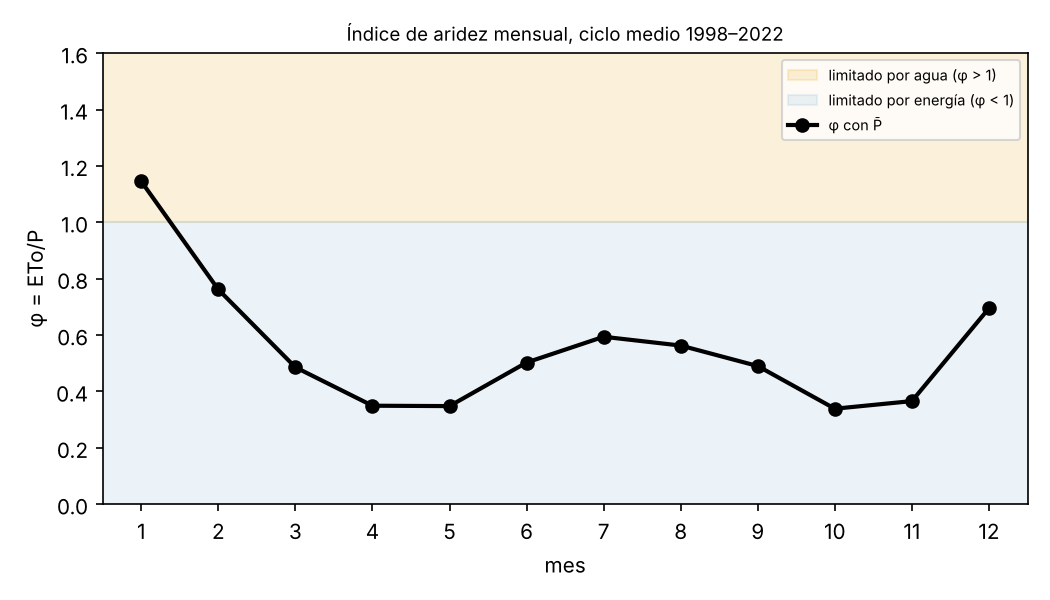
\includegraphics[width=0.48\textwidth]{regimen_mensual.png}\hfill
  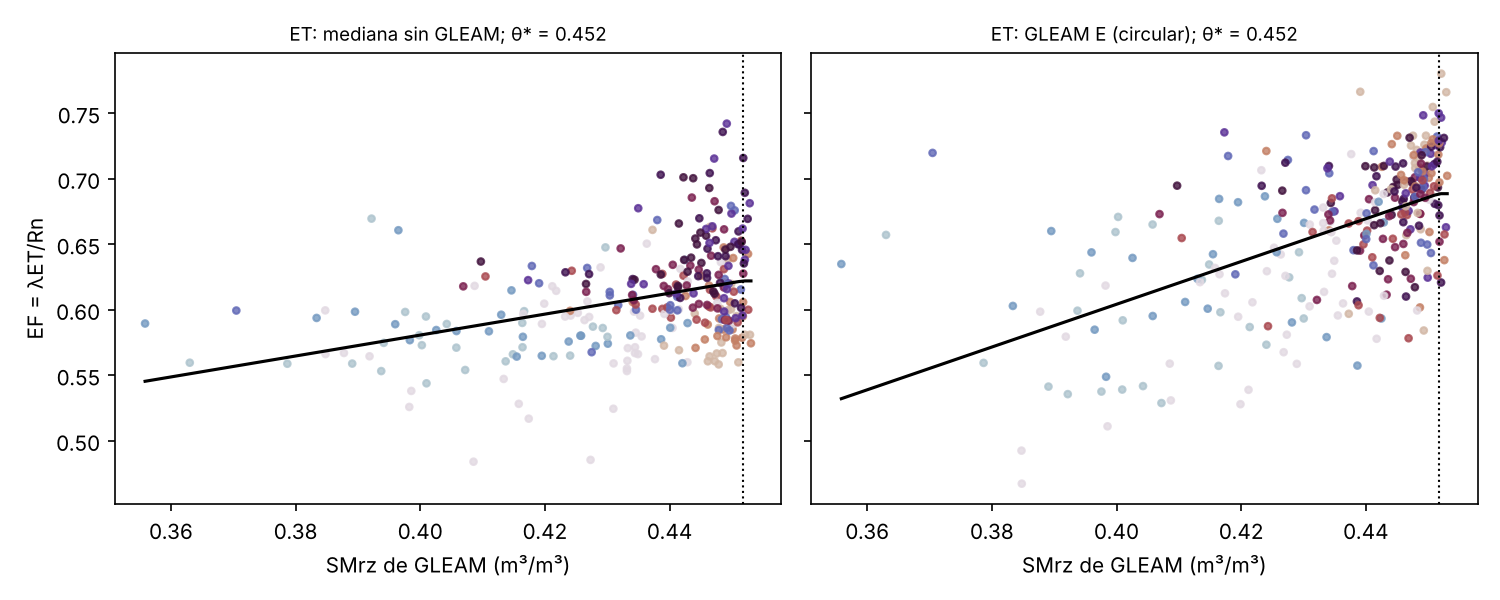
\includegraphics[width=0.48\textwidth]{fraccion_evaporativa.png}
  \caption{Izquierda: índice de aridez mensual $\varphi = \mathrm{ET_o}/\bar{P}$. Derecha: fracción evaporativa
  $\lambda\mathrm{ET}/R_n$ frente a la humedad del suelo de la zona de raíces de GLEAM.}
  \label{fig:regimen_ef}
\end{figure}
% Textos de Juan (temp/textos_informe/fase7_*.md).
Frente al índice de aridez (Fig.~\ref{fig:regimen_ef}), todos los meses en promedio son húmedos, con $\varphi < 1$,
menos enero, con $\varphi = 1.15$ en promedio y por encima de 1 más de la mitad de los años. Febrero es un poco más
árido que los demás. $\varphi > 1$ en un mes dice que la lluvia del mes no cubre la demanda, no que la ET esté
frenada: en enero el suelo amortigua.

La cuenca no está limitada por agua; está sobre todo limitada por energía. Si en algún mes estuviera limitada por
agua, se vería un quiebre en la fracción evaporativa, y no se ve: la ET es poco sensible a la humedad del suelo porque
el suelo casi siempre está húmedo. Esta prueba sola no es concluyente; se apoya también en Budyko
(Fig.~\ref{fig:budyko}) y en el índice de aridez mensual.
\pendiente{Juan: cifras de Budyko ($\varphi$, $\varepsilon$, $\omega$, elasticidad) y explicación alternativa.}

\subsubsection{Cambios en la demanda}
\begin{figure}[htbp]\centering
  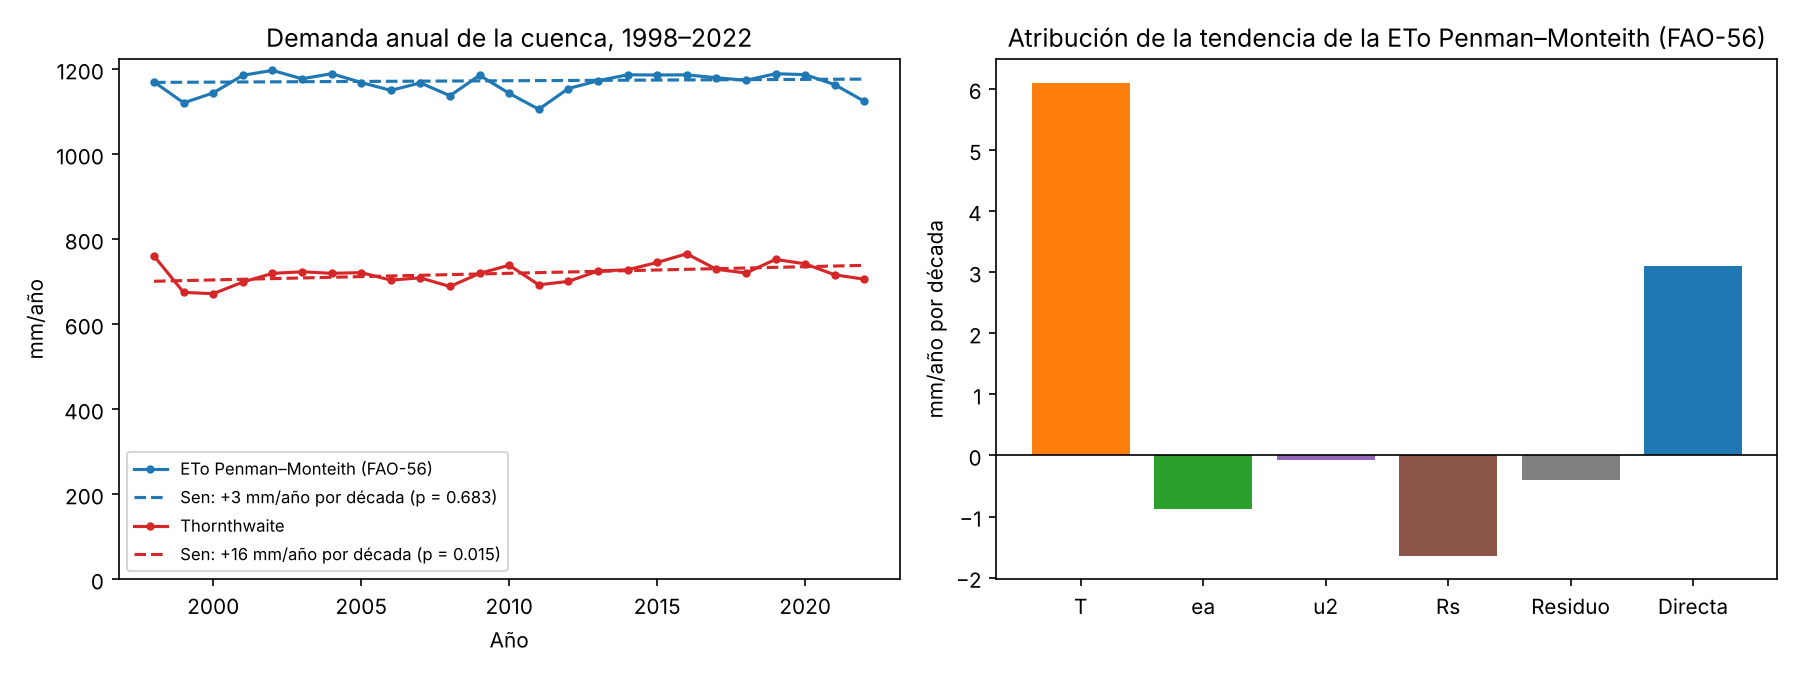
\includegraphics[width=\textwidth]{tendencias_demanda.png}
  \caption{Izquierda: \ETo{} \PM{} y Thornthwaite anuales con la recta de Sen, 1998--2022. Derecha: atribución de la
  tendencia de la \ETo{} a cada forzante.}
  \label{fig:tendencias}
\end{figure}
% Conclusión de Juan (temp/textos_informe/fase8_conclusion.md).
La \ETo{} \PM{} no tiene tendencia en 1998--2022 (Sen $+3$~mm/año por década, $p = 0.68$; Fig.~\ref{fig:tendencias}).
En Thornthwaite la tendencia es estadísticamente detectable con Mann-Kendall ($p = 0.015$), pero pequeña en magnitud:
$+16$~mm/año por década, cerca de 2~\% por década; OLS con Newey-West no la confirma ($p = 0.086$).

\subsubsection{El paisaje de la cuenca}
\pendiente{Fase 9: tema elegido y por qué se descartan los otros cinco.}

\subsection{Punto 2}
\pendiente{Resultados y recomendación de diseño con su incertidumbre (compañera).}

% =====================================================================================================
\section{Conclusiones}
\pendiente{Respuesta a las preguntas iniciales, sin repetir cifras ni traer resultados nuevos.}

% =====================================================================================================
\section{Uso de inteligencia artificial}
\pendiente{Declaración desde \texttt{anexos/bitacora\_ia.md}: herramientas y versión, tareas, qué se verificó y cómo,
qué se rechazó o corrigió y la contribución de cada integrante.}

\bibliographystyle{plainnat}
\bibliography{referencias}

\end{document}
